% !TEX root=../main.tex
\documentclass[beamer]{standalone}
\begin{document}

% Differentiable rendering
\begin{frame}{Background}
\framesubtitle{Differentiable rendering}

\begin{itemize}
    \item Differentiable rendering pipeline
    \begin{figure}[h]
        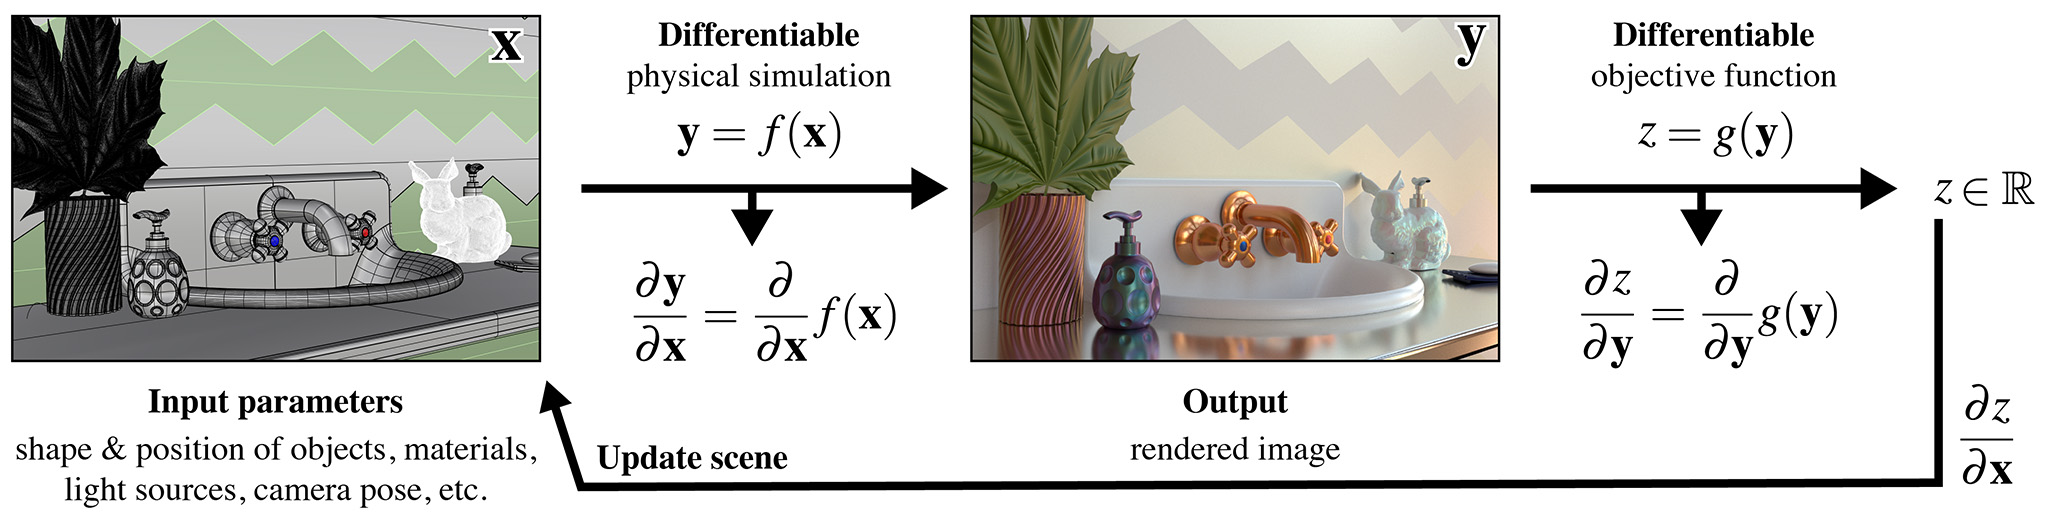
\includegraphics[width=0.8\linewidth]{figures/background-figure-2.jpeg}
        \caption{Mitsuba2: inverse rendering}
    \end{figure}
    \item Objective function
    \begin{enumerate}
        \item $ argmin \frac{1}{2} \left\lVert G.T. - R(x) \right\rVert^{2}  $
    \end{enumerate}

\end{itemize}

\note[item] {
    So, to understand this paper, we need at least two prior knowledges. The first one is differentiable rendering. 
    I will pass this part, because the previous presenter explain this sufficiently.
    }
\end{frame}

% Mesh propertices / laplace
\begin{frame}{Background}
\framesubtitle{Laplace operator}
\begin{itemize}
    \item Laplace operator
    \begin{enumerate}
        \item $ \mbox{\small $\Delta f = \diffp{f}{{x_{1}^{2}}} + \diffp{f}{{x_{2}^{2}}} + \cdots + \diffp{f}{{x_{n}^{2}}}$ } $
        \item Laplacian is deviation from local average
    \end{enumerate}

    \pause

    \item Discrete laplace operator on \small polygonal mesh $\mathcal{M} = (V, E)$
    \begin{enumerate}
        \item The weights $w_{ij} \in \mathbb{R} $ discretize the first derivative along an edge
        \item The addition of first derivatives within $L$ extends a second derivative to signals on $\mathcal{M}$
    \end{enumerate}
    \begin{figure}[h]
        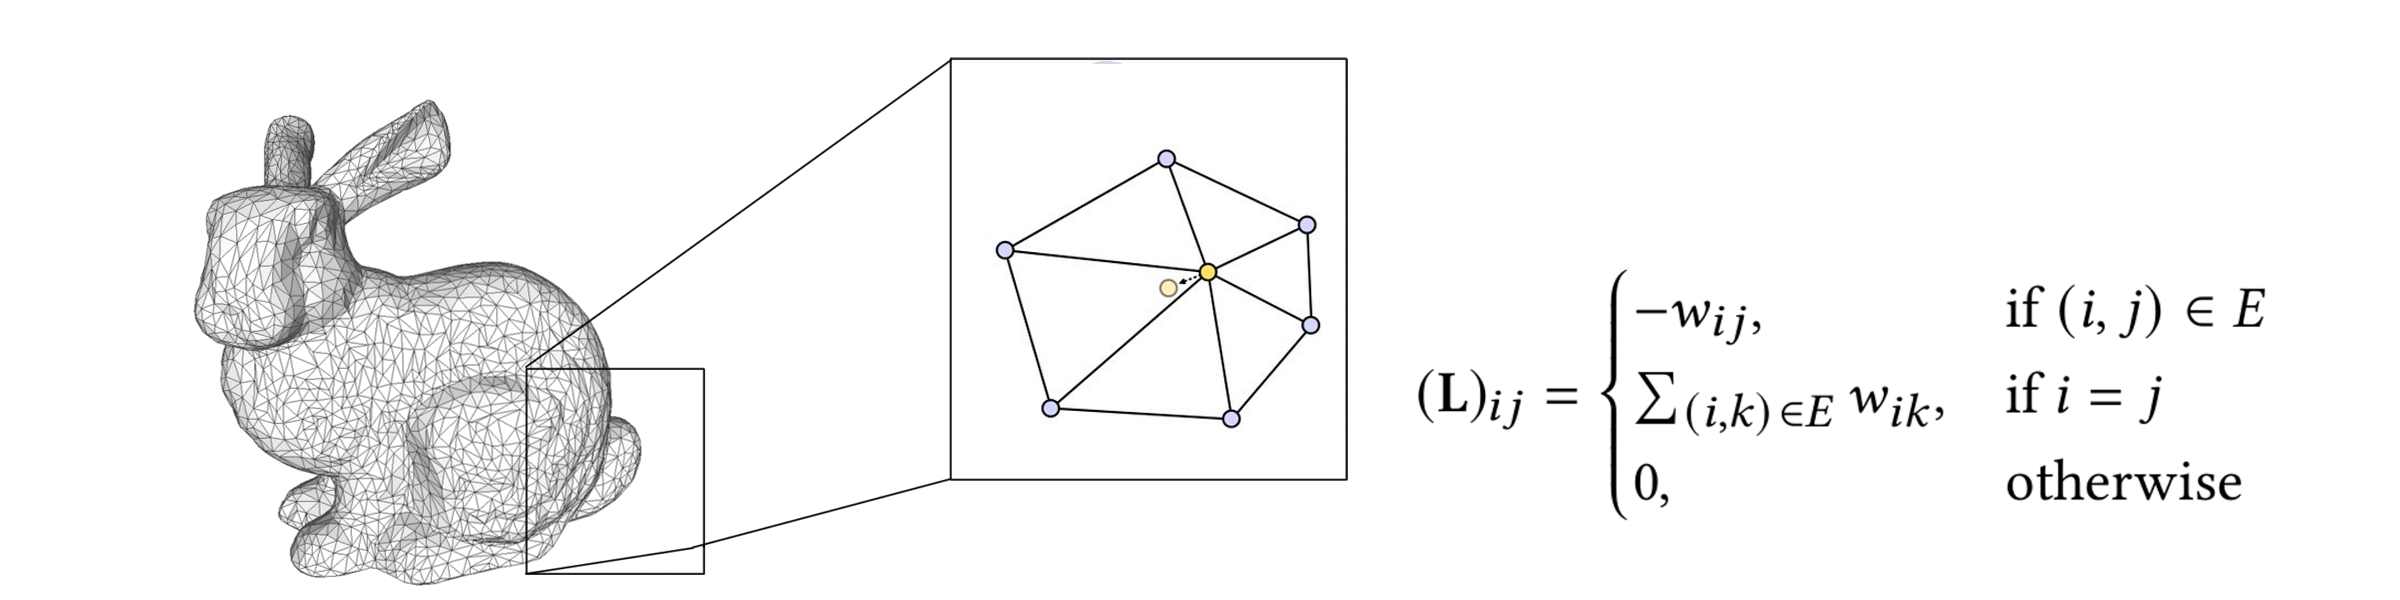
\includegraphics[width=0.8\linewidth]{figures/background-figure-3.png}
    \end{figure}

    \pause

    \item Laplace regularaizer
    \begin{equation}
        minimize_{x\in\mathbb{R}^{nX3}}  \; \Phi(R(x)) + \textcolor{red}{\frac{\lambda}{2} tr(x^{T}Lx)}
    \end{equation}
\end{itemize}
    
% notes %
\note[item]{
    The second one is laplace operator.

    The laplace operator looks like this. To easily understand, laplacian indicate the deviation from local average.
    That means, in the specific point, how spiky that point is along the local area.

    On polygonal mesh, we can think laplacian similar as Graph Laplacian.
    On Laplace operator, the weights is the discretized version of the first derivatie along the an edge.
    Therefore, we can interpret the addition of first derivative of laplacian as a second derivate of signal on mesh.
    
    Then, it can be said that a laplace regularizer wants each vertex to be at the center of its neighbors.
    So it is a compromise for the original objective function.
    }   
\end{frame}

\end{document}
